\documentclass[14pt,fleqn]{extarticle}
\RequirePackage{prepwell}
\previewoff
\begin{document}

%text
A die is thrown again and again until three 
sixes are obtained. Find the probability of 
obtaining the third six in the sixth throw 
of the dice.
%

\newcard

\begin{center}
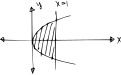
\includegraphics[scale=0.7]{right.svg} 
\end{center} 

\newcard

\begin{center}
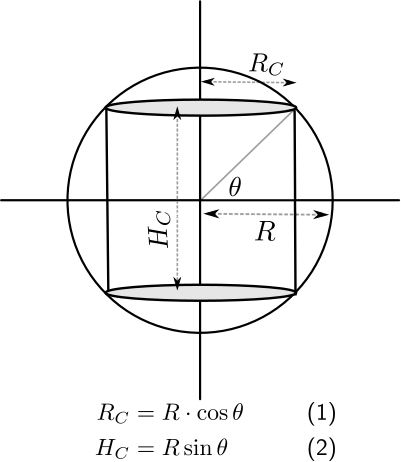
\includegraphics[scale=0.7]{wrong.svg}
\end{center} 

\newcard

Any favourable outcome will have the following characteristics 

\begin{itemize}
\item{The last throw will be a 6} 
\item{There will be \underline{exactly} two 6's in throws 1-5} 
\end{itemize} 

Which is why, a favourable outcome would look like the figure below. 
But it is not the only favourable outcome. There are more. 

\begin{center}
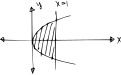
\includegraphics[scale=0.7]{right.svg}  
\end{center} 

\newcard 

The required probability $P$ is therefore 
\[ P = \left[^5C_2\cdot\left(\frac{1}{6} \right)^2\cdot\left(\frac{5}{6}\right)^3\right]\times\frac{1}{6}=\frac{625}{23328} \]

\newcard

The required probability $P$ is therefore 
\[ P = {^6C_3}\cdot\left(\frac{1}{6} \right)^3\cdot\left(\frac{5}{6}\right)^3=\frac{625}{11664} \]

\newcard

We would get a favourable outcome if the following happens 

%
\begin{center}
\begin{tabular}{NNN}
\toprule
\text{Throws} & \text{Requirement} & \text{\# of ways} \\
\midrule 
1-5 & \text{Exactly two sixes} & ^5C_2 \\
\midrule 
6 & \text{A six} & 1 \\
\bottomrule 
\end{tabular}
\end{center} 
%text

Hence, the \underline{required probability} will be 
%
\begin{align}
P &\left(\text{getting a six} \right) = p = \frac{1}{6}\\
\implies P &\left(\text{not getting a six} \right) = q = \frac{5}{6} \\
\therefore P &= \underbrace{^5C_2\cdot p^2\cdot q^3}_{\text{Throws 1-5}}\times\underbrace{p}_{\text{Last throw}} \\
\implies P &= \left[^5C_2\cdot\left(\frac{1}{6} \right)^2\cdot\left(\frac{5}{6}\right)^3\right]\times\frac{1}{6} = \frac{625}{23328}
\end{align}

\end{document}
